% !TeX encoding = UTF-8
% !TeX program = xelatex
% !TeX spellcheck = fr
% !TeX root = tm_astro_main.tex

\chapterFormatfive

\chapter{Enrichissement du milieu interstellaire}\label{5}

\chapterFormat

Comme nous l'avons vu dans les chapitres \ref{2} et \ref{3}, des éléments lourds sont produits par les étoiles au cour de leur fin de vie. Ces éléments peuvent de différentes manières se retrouver séparer de leur étoile. Les vents stellaires incarnent l'une des ces manières; en effet les étoiles AGB (§\ref{2.2.2}) ainsi que les supergéantes (§\ref{2.4}) sont balayées par de forts vents parvenant à retirer jusqu'à plusieurs masses solaires de matière à l'étoile. Les nébuleuses planétaires (§\ref{2.3}) et les supernovas (§\ref{3}) représentent une autre méthode pour expulser dans le milieu interstellaire les composants d'une étoile. Ces deux phénomènes mettent le coeur d'une étoile à nu; toute la matière constituant les anciennes couches supérieures de l'étoile est maintenant éjectée dans le vide interstellaire. 

\section{Evolution et rôle du milieu interstellaire}\label{5.1}

Au fil du temps, des nuages de gaz enrichis par la matière d'anciennes étoiles se forment: les nébuleuses. Ces objets célestes possèdent un rôle majeur dans la naissance des étoiles; on les surnomme d'ailleurs les pouponnières d'étoiles. Les composants du gaz de la nébuleuse se rapprochent les uns des autres sous l'effet de la gravitation jusqu'à former une boule de gaz, nous disons que le gaz s'effondre. En même temps que la pression du gaz croît, la température augmente; arrivé à un certain stade, la température est suffisante pour déclencher la fusion de l'hydrogène, une étoile est alors née. Au tour de la jeune étoile se trouve toujours un nuage de gaz, appelé disque protoplanétaire. A partir de celui-ci, des poussières interstellaires commencent à s'agréger. Les différents agrégats accrètent progressivement la matière du disque protoplanétaire. Au fur et à mesure, des exoplanètes se forment et le disque disparaît. En fonction de la composition initial du gaz différentes planètes sont créées. Par exemple, les planètes telluriques, comme la Terre, sont principalement constituée de silicium et de fer; Jupiter, quant à elle, est quasi intégralement composée d'hydrogène et d'hélium. De nos jours, nous savons donc que sans un milieu interstellaire enrichi par des générations entière d'étoiles les éléments nécessaires à l'apparition de la vie n'auraient jamais été réunis. La célèbre citation de l'astrophysicien Hubert Reeves résume parfaitement ce dernier paragraphe: << On m'a dit: tu n'es que cendre et poussières. On a oublié de me dire qu'il s'agissait de poussières d'étoiles.>>

\begin{figure}[H]
	\centering
	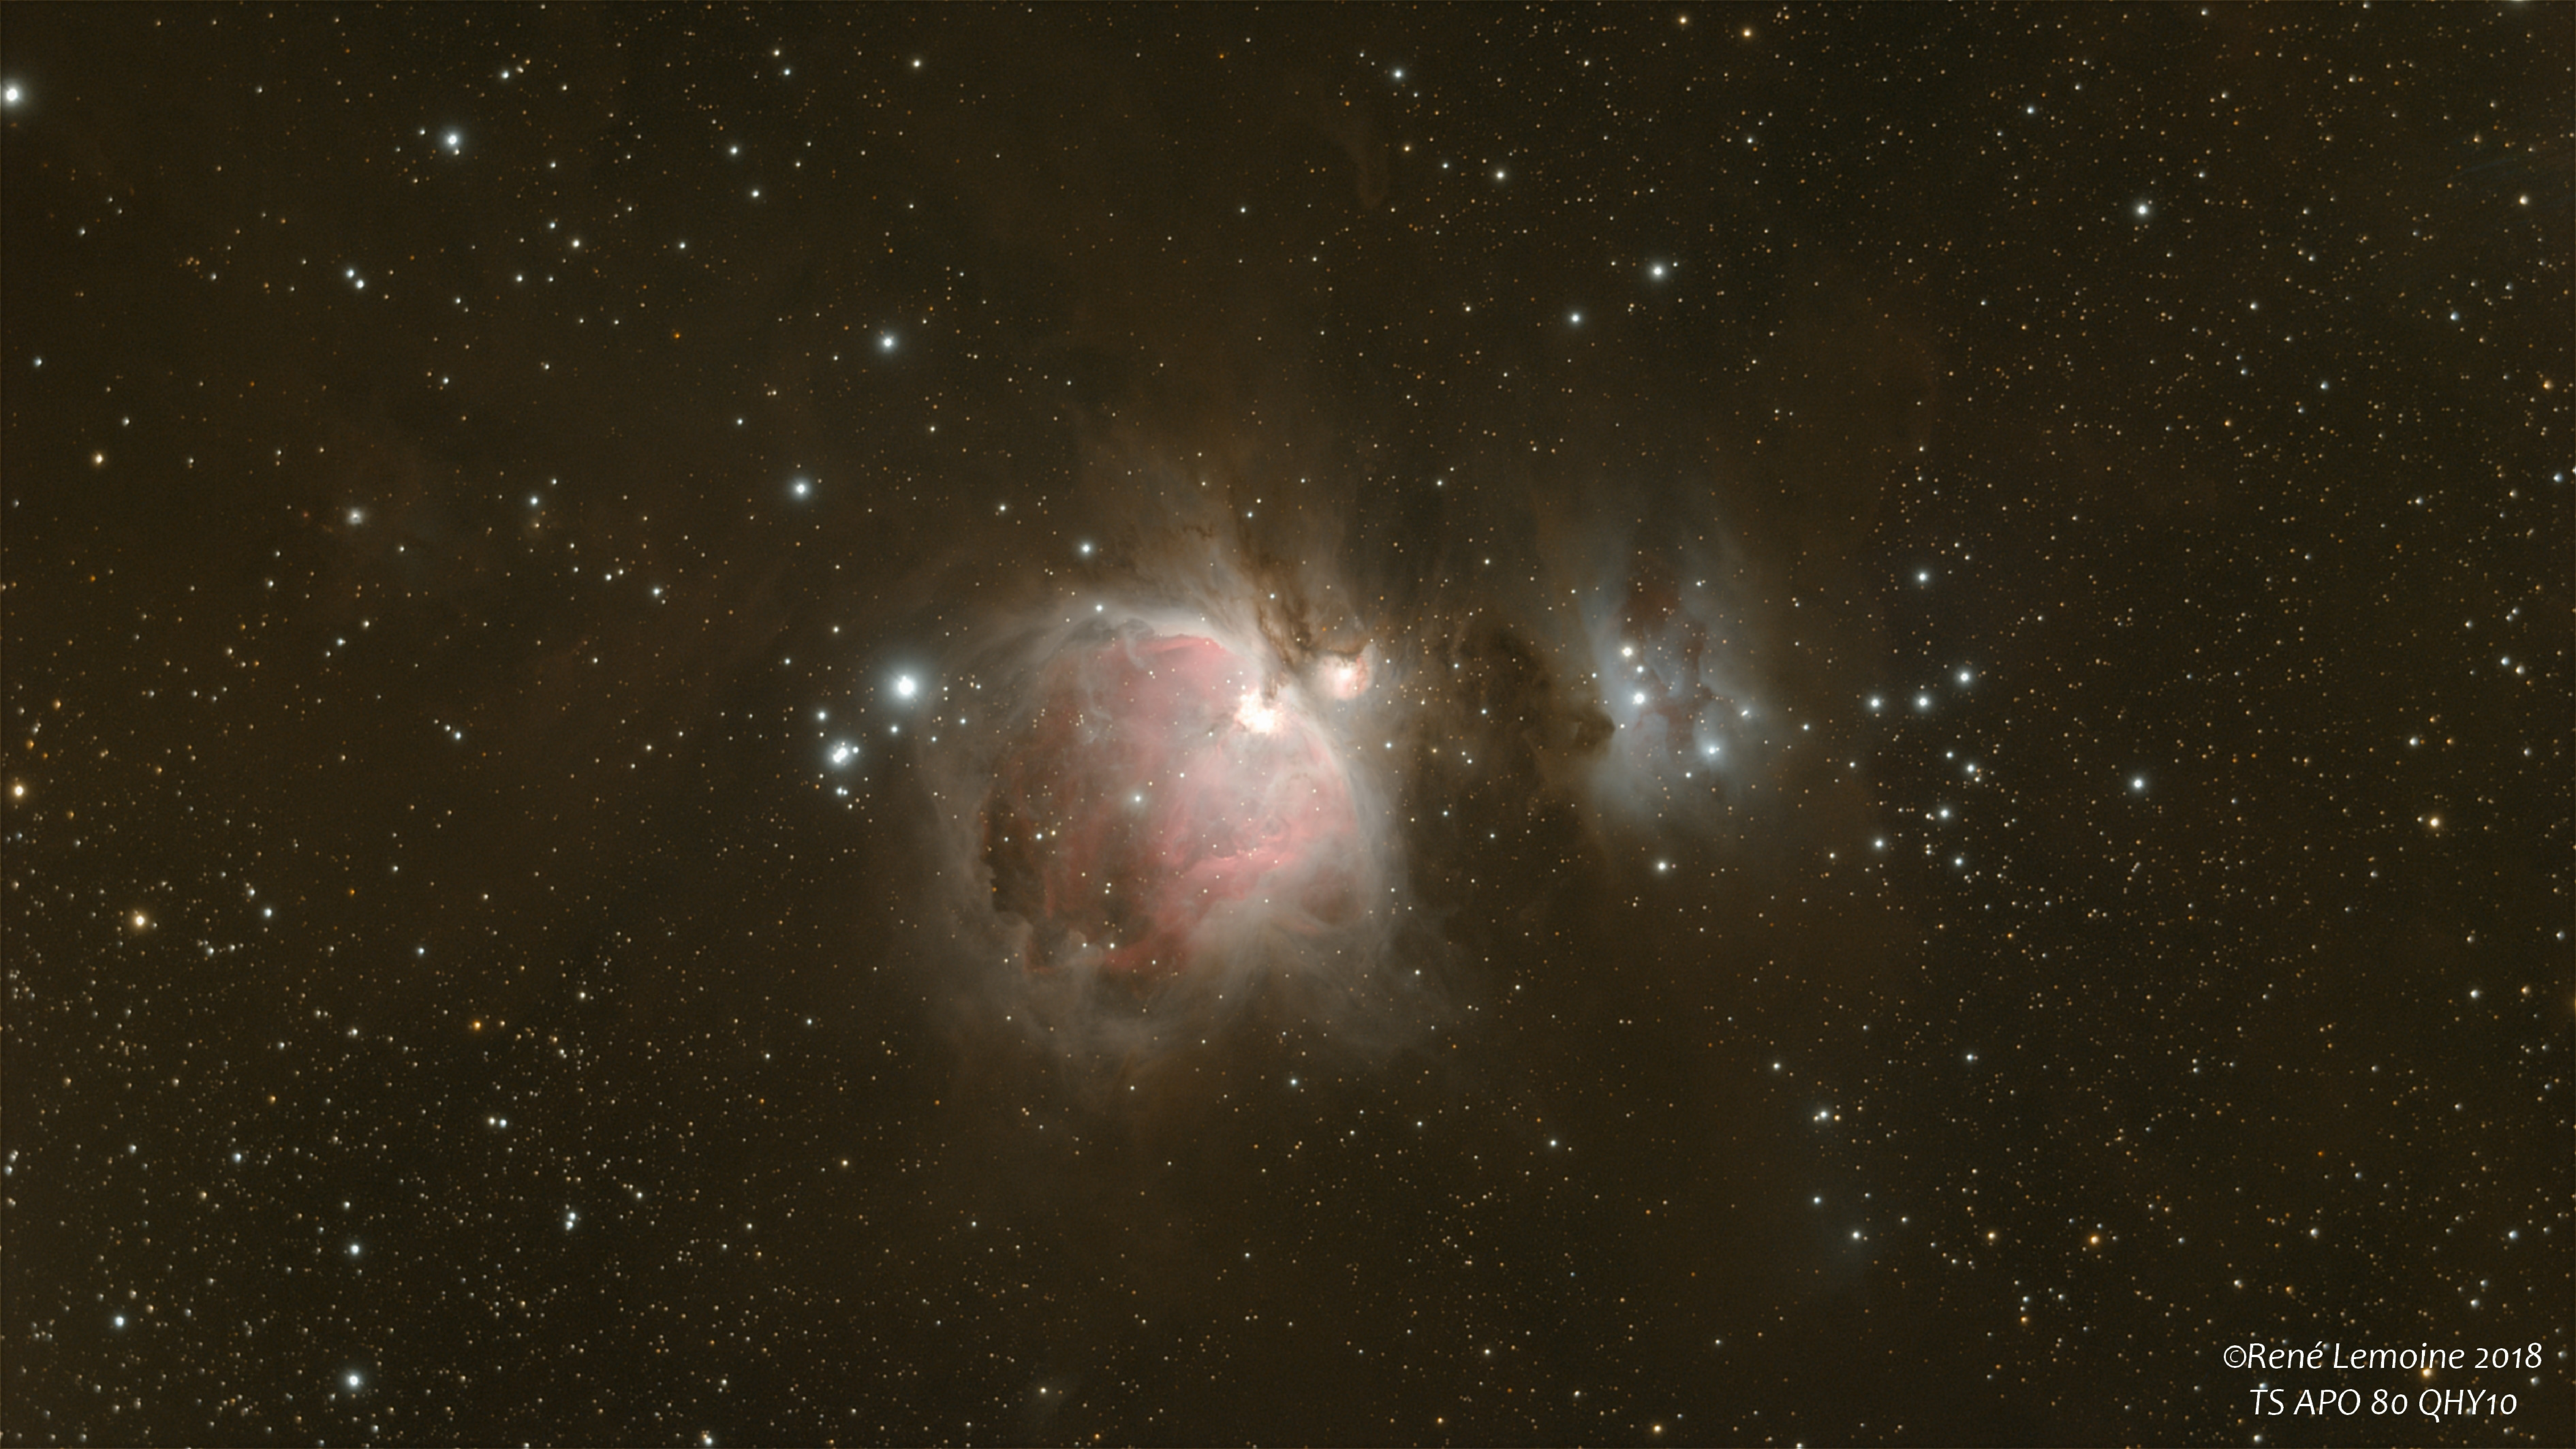
\includegraphics[scale=0.06]{images/orion}
	\caption[M42, nébuleuse d'Orion - astrophoto prise par René Lemoine en 2018 avec une lunette TS APO 80 et une caméra QHY10 (5 heures de pose)]{M42, nébuleuse d'Orion}
	\label{Fig. 5.1}
\end{figure}\bigskip



\section{ L'E-ELT dans ce domaine}\label{5.2}

Dans cette dernière section, nous allons traiter plus en profondeur des avancées attendues par l'E-ELT dans l'étude du milieu interstellaire. Dans un premier temps nous nous attarderons plus spécifiquement sur l'observation de rémanent de supernova. Ensuite, comme nous avons déjà quelque peu parler des exoplanètes dans la section \ref{5.1} il est intéressant d'aborder l'amélioration de leurs observations par le télescope géant européen.\medskip

L'E-ELT sera particulièrement performant dans l'observation des supernovas de type Ia (§\ref{3.1.2}) à haut décalage vers le rouge. Ce type particulier est privilégié car une des caractéristiques principales des supernovas de type Ia est la présence de raies de silicium dans leur spectre électromagnétique. Ce sera le spectrographe HARMONI (§\ref{4.2}), muni d'une optique adaptative, qui sera principalement chargé de cette mission. Le télescope géant européen révolutionnera ce domaine d'étude dans le mesure où il sera capable d'observer des décalages dans le rouge plus élevé que ceux observer avec d'autres télescopes déjà existant. Le fait que ces objets soient décalés vers le rouge signifie qu'ils s'éloignent de nous à grande vitesse; cela est dû à l'expansion de l'univers, qui de plus est accélérée. En d'autres termes, cela signifie que plus les objets sont distancés de nous, plus ils s'éloignent rapidement. De plus, comme la vitesse de la lumière est finie (même si elle est très grande), tout ce que nous observons n'est pas dans le présent, mais plutôt dans un passé plus ou moins lointain. Ainsi si nous recombinons ce que l'on vient dire on arrive à la conclusion que plus on regarde décalé dans le rouge plus on regarde dans le passé. C'est grâce à ce phénomène que l'E-ELT aura la capacité d'observer des évènements qui se sont passés dans le premier dixième de la vie de notre univers. A titre d'information, les meilleurs télescopes à ce jour sont capables de "remonter" jusqu'à environ la moitié de l'âge de notre univers. Il est intéressant de pouvoir analyser des évènements toujours de plus en plus éloigné dans le temps afin, d'une part augmenter notre niveau de compréhension de l'évolution primordiale de l'univers et, d'une autre part apporter de nouvelles pistes aux théories traitant de sa création.\medskip

La recherche et l'étude des exoplanètes est l'un des principaux domaines de l'astronomie moderne. Ce secteur de recherche bénéficie d'un grand appui budgétaire notamment grâce à ses objectifs scientifiques: la recherches de planètes potentiellement habitables et la découverte d'une possible vie extraterrestre. De nombreux télescopes terrestres et spatiaux ont pour objectif de découvrir, recenser ou encore analyser des exoplanètes. L'E-ELT ne déroge pas à cette règle avec son instrument HARMONI (§\ref{4.2}). Les télescopes existants qui étudient les exoplanètes utilisent principalement des techniques indirectes pour les détecter. Ces méthodes recherchent l'influence que possède une exoplanète sur son étoile hôte. Cette influence peut se manifester par des petites variations de luminosité (méthode des transits) ou bien encore par des variations de la vitesse radiale d'une étoile (méthode des vitesses radiales). Grâce à sa très grande résolution, l'E-ELT sera capable de tirer son épingle du jeu en observant directement certaines exoplanètes sans passer par des méthodes indirectes. De plus, son spectrographe aura la capacité d'identifier avec précision des molécules chimiques présentes dans des atmosphères d'exoplanètes relativement proches de nous. Dans notre quête de la découverte d'une vie extraterrestre, nous essayons de mettre la main sur des exoplanètes possédant les mêmes caractéristiques que la Terre. En détectant les mêmes molécules qui ont permis l'apparition de la vie sur notre planète (comme l'eau H$_{2} 0$ ou encore le dyoxygène $0_{2}$) et en remplissant d'autres critères qui rendrait cette exoplanète semblable à la nôtre, il y aurait peut-être une infime chance qu'une forme de vie équivalente à la nôtre ait pu se développer. Le problème se trouve dans le fait qu'en choisissant la Terre comme modèle de recherche, nous restreignons grandement le nombre de candidats à abriter la vie. D'une certaine manière, la vie existe peut-être ailleurs mais sous une toute autre forme que nous imaginons.










